% Ejercicio 3 (2): grafica de g(x,y) = cos(2x) sen(y) sobre
% [-pi/2, pi/2] x [-pi, pi], que contiene un periodo completo en cada variable.
% Los maximos (valor 1) estan en (0, pi/2) y (+-pi/2, -pi/2), los minimos
% (valor -1) en (0, -pi/2) y (+-pi/2, pi/2), y las sillas (valor 0) en
% (+-pi/4, k pi).
\documentclass[tikz,border=3pt]{standalone}
\usepackage{pgfplots}
\pgfplotsset{compat=1.18}
\begin{document}
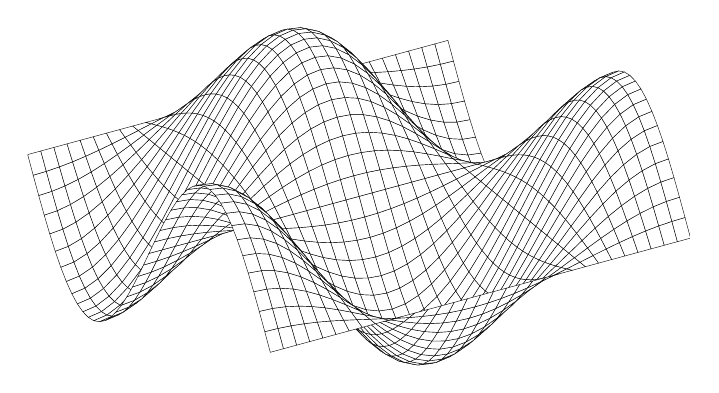
\begin{tikzpicture}
  \begin{axis}[
      hide axis,
      view={-30}{40},
      width=10cm, height=9cm,
      domain=-pi/2:pi/2, y domain=-pi:pi,
      samples=33, samples y=45,
      z buffer=sort,
    ]
    \addplot3[surf, shader=faceted, faceted color=black, fill=white,
      opacity=1, line width=0.15pt]
      ({x},{y},{cos(deg(2*x))*sin(deg(y))});
  \end{axis}
\end{tikzpicture}
\end{document}
